% !TeX program = xelatex
% !TeX encoding = UTF-8
%
% 中文对照稿。请从本目录使用 XeLaTeX 编译。
% 共用上一级目录中的 Elsevier CAS 类、图件和参考文献文件。
% 基于 Elsevier CAS Bundle 的单栏模板，其模板按 LPPL 1.3c 或更高版本分发。

\makeatletter
\def\input@path{{../}}
\makeatother
\PassOptionsToPackage{nomath}{stix}
\documentclass[a4paper,fleqn]{cas-sc}
\usepackage[UTF8,scheme=plain,fontset=fandol]{ctex}
\usepackage[numbers,sort&compress]{natbib}
% 使用 XeLaTeX 的 OpenType 数学字体，避免 CAS 旧版数学符号错位。
\usepackage{unicode-math}
\setmathfont{STIXTwoMath-Regular.otf}
\graphicspath{{../}}
\renewcommand{\sfdefault}{\rmdefault}
\urlstyle{same}

\renewcommand{\abstractname}{摘\quad 要}
\renewcommand{\figurename}{图}
\renewcommand{\tablename}{表}
\renewcommand{\refname}{参考文献}

\newcommand{\sectionbudget}[2][初稿可供审阅]{%
  \noindent{\small\textbf{版面预算}\enspace 约 #2 页\quad
    \textbf{状态}\enspace #1}\par\nobreak
}
\newcommand{\subsectionbudget}[1]{%
  \noindent{\small\textbf{版面预算}\enspace 约 #1 页}\par\nobreak
}

\definecolor{guideblue}{HTML}{35678F}
\newlength{\displayguidewidth}
\newcommand{\displayguide}[5]{%
  \begingroup
  \setlength{\displayguidewidth}{#1}%
  \setlength{\fboxrule}{0.7pt}%
  \setlength{\fboxsep}{6pt}%
  \noindent\fcolorbox{guideblue}{guideblue!6!white}{%
    \begin{minipage}{\dimexpr\displayguidewidth-2\fboxsep-2\fboxrule\relax}
      \hypersetup{linkcolor=black}%
      \raggedright\small
      {\color{guideblue}\bfseries #2\par}\smallskip
      \textbf{所需数据}\enspace #3\par
      \textbf{制作要点}\enspace #4\par
      \textbf{验收标准}\enspace #5\par
    \end{minipage}}%
  \endgroup\par\medskip}
\newcommand{\figureguide}{\displayguide{\dimexpr.88\linewidth+2\fboxsep+2\fboxrule\relax}}

% 在首页标题与文字摘要之间插入图文摘要。
\BeforeBeginEnvironment{Abstract}{%
  \par
  \begingroup
  \vspace{5pt}%
  \noindent 图文摘要\par
  \dashrule[.2pt]{2pt}{5pt}%
  \noindent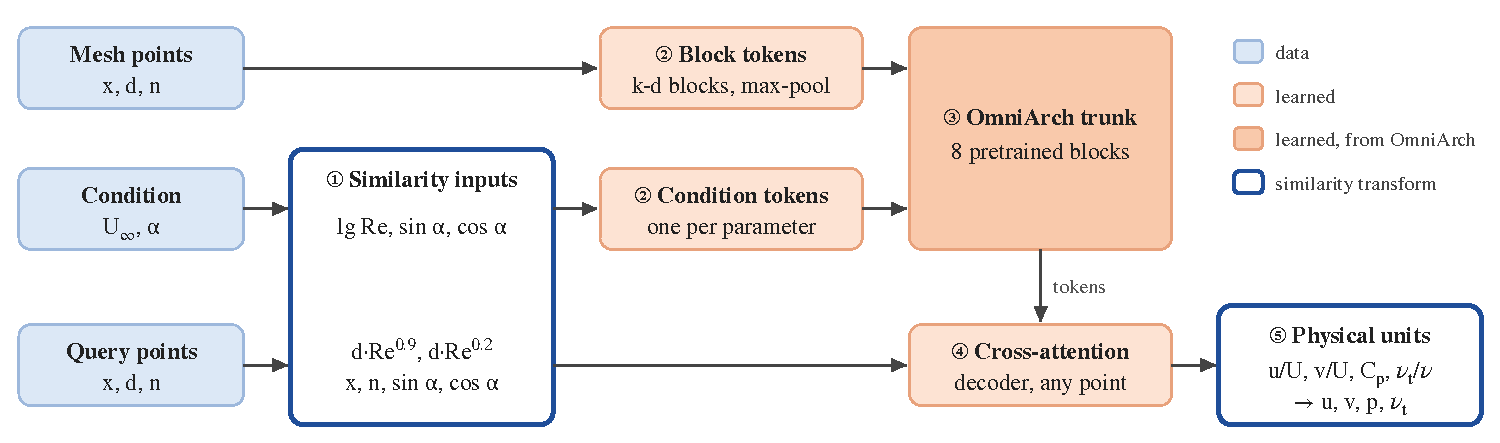
\includegraphics[width=.5\linewidth]{figs/overview.pdf}\par
  \dashrule{5pt}{10pt}%
  \endgroup
}

\begin{document}
\let\WriteBookmarks\relax
\def\floatpagepagefraction{1}
\def\textpagefraction{.001}

\shorttitle{}
\shortauthors{}
\title[mode=title]{面向翼型流场与涡轮叶片温度相似外推的 OmniArch 模型适配}

% 作者和单位可直接输入中文。
% \author[1]{作者姓名}
% \affiliation[1]{organization={单位名称},city={城市},country={中国}}
% \cormark[1]
% \ead{author@example.com}
% \cortext[1]{通信作者}

\begin{abstract}
计算流体力学是飞行器与发动机设计的基础。设计评估需要在多种工况下考察每个候选方案，因此代理模型既要推理迅速，又要在超出训练范围的工况下保持精度。现有方法在这两项要求之间存在取舍。传统数值求解器根据控制方程逐个求解，每个工况通常耗时数分钟至数小时，在极端工况下还可能不收敛或失准。神经算子可以在毫秒量级完成预测，但雷诺数或温度超出训练范围时，预测精度会下降。量纲分析可以用少数相似变量描述尺度变化，既有应用多涉及标量，较少涉及非结构网格上的全场预测。

本文提出相似特化方法，用控制方程中的相似变量重写预训练偏微分方程基础模型的输入和输出。其思路与风洞试验的缩比换算相似，通过相似变量将训练工况中学到的规律用于新工况，并让模型学习相似律未覆盖的尺度效应。在相似变量下，有量纲参数的外推在很大程度上可转化为内插。据此构建 OmniArch-Aero，将非结构网格划分为空间块并编码为 token，由预训练的 OmniArch 主干处理，再用交叉注意力在任意查询点解码物理场。

在 AirfRANS 雷诺数外推任务上，OmniArch-Aero 的升力系数误差较已发表的最佳模型降低 91\%。单个工况的流场预测耗时 \(0.22\,\mathrm{s}\)，RANS 求解耗时约 \(25\,\mathrm{min}\)。这些结果提示，物理感知基础模型宜在相似变量空间中学习。
\end{abstract}

\begin{keywords}[关键词]
量纲分析 \sep
偏微分方程基础模型 \sep
非结构网格 \sep
参数外推 \sep
翼型空气动力学 \sep
涡轮叶片冷却
\end{keywords}

\maketitle

\section{引言}\label{sec:introduction}
\sectionbudget{2}

同一气动或热设计往往需要在多种运行工况下进行评价。对于翼型，近壁流场和表面压力决定了评价气动性能所需的载荷。对于冷却涡轮叶片，金属温度场用于辨识高温区域并评估热裕度\citep{Han2013}。每增加一个工况，通常都需要重新求解控制方程，叶片算例还涉及流体与固体的共轭传热计算。代理模型可以复用已有数值解来降低这一成本\citep{Brunton2020,Benner2015}。它能否用于超出已有样本范围的工况，取决于能否恢复该工况的物理场及其对应的工程量。

傅里叶神经算子（FNO）和 DeepONet 等方法通过学习函数间的映射，近似一族参数化偏微分方程的解\citep{Li2021FNO,Lu2021DeepONet}。Transolver 等考虑几何信息的方法将算子学习扩展到复杂几何\citep{Wu2024Transolver}。OmniArch 等科学计算基础模型提供了可用于下游任务初始化的预训练参数\citep{Chen2025OmniArch}。这些进展为不规则计算域上的全场预测提供了模型基础。本文关注的问题是，当给定几何和工况中的雷诺数或进口温度超出训练范围时，代理模型能以怎样的精度预测物理场。

量纲分析可以区分物理尺度的变化与解结构的变化。Buckingham \(\Pi\) 定理给出了将有量纲变量组合为无量纲群的方法\citep{Buckingham1914}。Bakarji 等利用数据识别相关的无量纲群\citep{Bakarji2022}，Oppenheimer 等将无量纲变量用于跨尺度学习\citep{Oppenheimer2023}。这些研究为用特征尺度表示工况与预测场提供了依据。对于非结构网格上的预训练代理模型，需要进一步确定哪些尺度可以显式处理，以及哪些随工况发生的变化需要利用已有参考解学习。

两个应用所需的相似变量不同。在翼型绕流中，来流速度 \(U_\infty\) 决定了速度和运动压力的特征尺度，分别为 \(U_\infty\) 和 \(U_\infty^2\)。雷诺数仍影响无量纲动量平衡，因此模型还需描述其对缩放后流场的影响。对于叶片，主流与冷气进口总温之差为金属温度场提供了温度尺度。已有研究从理论和冷却导向叶片试验两方面考察了金属温度的相似缩放\citep{Luque2016,Luque2017}。整体冷却有效度也会随进口温度比和燃气物性变化\citep{Cartlidge2024}。对于固定叶片网格，可以利用较低温度下的参考场，在对应节点处估计无量纲温度随工况的变化。

本文构建 OmniArch-Aero，将面向任务的相似表示用于非结构网格上的场预测。网络将网格编码为空间块，使用由 OmniArch 预训练参数初始化的主干处理块 token，再在查询点解码物理场。对翼型任务，利用相似变换定义工况输入与流场预测量。对冷却叶片任务，用低温参考场拟合逐节点温度先验，并由网络学习残差修正。两项任务采用同一架构并分别训练。物理问题与相似变换分别见第~\ref{sec:problem-statement}~章和第~\ref{sec:methodology}~章。

第~\ref{sec:airfrans-results}~章基于 AirfRANS 数据集\citep{Bonnet2022AirfRANS}，在训练区间以外的雷诺数工况上比较有量纲配置与相似配置，并用预测场恢复的升力评价气动力精度。第~\ref{sec:blade-results}~章在固定叶片几何和网格上比较直接相似换算、逐节点温度先验以及先验与网络残差的组合，分别量化低温先验和残差修正对两个高温测试工况温度预测的贡献。

\section{问题描述}\label{sec:problem-statement}
\sectionbudget{2}

本文考察多种翼型的雷诺数外推，并在主流进口总温超出训练范围时预测同一冷却涡轮叶片的温度场。

\subsection{翼型流动与雷诺数外推}\label{subsec:airfoil-problem}
\subsectionbudget{1.00}

考虑二维稳态不可压缩翼型绕流。翼型弦长为 $L$，来流速度大小为 $U_\infty$，方向由攻角 $\alpha$ 描述。本文以 AirfRANS 数据集的雷诺平均 Navier--Stokes（RANS）数值解为参考场。假定流体密度 $\rho$ 和运动黏度 $\nu$ 为常数，并忽略体力。取 $L$ 和 $U_\infty$ 为特征尺度，流体域中的无量纲质量与动量方程\citep{Pope2000}为
\begin{equation}
  \label{eq:airfoil-rans}
  \begin{aligned}
    \nabla^*\!\cdot\mathbf{u}^* &= 0, \\
    (\mathbf{u}^*\!\cdot\nabla^*)\mathbf{u}^*
      &= -\nabla^*p^*
         + \frac{1}{Re}\nabla^{*2}\mathbf{u}^*
         - \nabla^*\!\cdot\mathbf{R}^*,
         \qquad Re=\frac{U_\infty L}{\nu}.
  \end{aligned}
\end{equation}

这里，$\mathbf{x}^*=\mathbf{x}/L$，$\nabla^*$ 表示对 $\mathbf{x}^*$ 求导，$\mathbf{u}^*=\overline{\mathbf{u}}/U_\infty$。无量纲压力为 $p^*=(\overline{p}-p_{\mathrm{ref}})/(\rho U_\infty^2)$，其中 $p_{\mathrm{ref}}$ 为参考压力。无量纲雷诺应力张量为 $\mathbf{R}^*=\overline{\mathbf{u}'\otimes\mathbf{u}'}/U_\infty^2$，$\mathbf{u}'$ 为速度脉动。式~\eqref{eq:airfoil-rans} 中的系数 $1/Re$ 决定分子黏性项在无量纲动量平衡中的相对权重，因此无量纲流场仍可随雷诺数变化。AirfRANS 参考解采用 $k\!-\!\omega$ SST 湍流模型闭合 RANS 方程，并在翼型壁面施加无滑移条件\citep{Bonnet2022AirfRANS}。

给定翼型的非结构网格及来流工况，模型预测每个网格节点上的 $(u,v,p_{\mathrm{kin}},\nu_t)$。其中 $u$、$v$ 为平均速度的两个分量，$p_{\mathrm{kin}}$ 为运动压力，即按数据集压力基准表示的平均压力除以密度，$\nu_t$ 为湍流运动黏度。以节点物理场作为监督目标，相应的变量变换和训练设置分别见第~\ref{subsec:airfoil-similarity}~节和第~\ref{subsec:mesh-to-field}~节。为评价预测场对整体气动力的描述，由壁面压力与黏性剪切计算升力系数 $C_L$，并与参考解得到的升力系数比较。

外推试验按雷诺数划分算例。训练样本的雷诺数位于 $[3\times 10^6,\,5\times 10^6]$，分别用低于训练下限和高于训练上限的工况检验区间外预测。各算例仍提供对应的翼型几何和攻角。第~\ref{subsec:airfrans-setup}~节介绍数据划分，第~\ref{subsec:airfrans-errors}~节评价升力预测精度。

\subsection{冷却叶片与温度工况外推}\label{subsec:blade-problem}
\subsectionbudget{1.00}

考虑一片带有冷却结构的涡轮转子叶片，记其固体域为 $\Omega_{\mathrm{s}}$。主流侧和冷气侧的界面热通量与固体内部的导热共同决定金属温度分布。给定叶片网格与工况，本文预测 $\mathbf{x}\in\Omega_{\mathrm{s}}$ 处的金属温度 $T(\mathbf{x})$，以 CFX 共轭传热计算得到的固体节点温度为参考解。各参考算例记录了主流与冷气的进口总温、两股气流的质量流量、出口静压和转速。

跨温度工况比较时，用冷热进口总温之差作为温度尺度。令 $T_g$ 和 $T_c$ 分别为静止参考系下的主流和冷气进口总温，则固体节点的无量纲温度 $\theta(\mathbf{x})$ 及其对应的金属温度为
\begin{equation}
  \label{eq:blade-temperature-similarity}
  \theta(\mathbf{x})=\frac{T_g-T(\mathbf{x})}{T_g-T_c},
  \qquad
  T(\mathbf{x})=T_g-(T_g-T_c)\,\theta(\mathbf{x}).
\end{equation}
记低温参考工况的无量纲温度为 $\theta_{\mathrm{ref}}(\mathbf{x})$。第~\ref{subsec:blade-setup}~节的直接相似基线在目标工况沿用这一分布，并将目标工况的 $T_g$ 和 $T_c$ 代入式~\eqref{eq:blade-temperature-similarity} 的逆变换以恢复金属温度。该基线处理的是进口温差尺度的变化。随温度变化的物性可能改变固体导热和流固界面换热，进而改变 $\theta$ 的分布。第~\ref{subsec:blade-prior}~节引入温度先验以描述这部分变化。

各工况共用同一叶片和同一套网格，固体节点的坐标一一对应，可以逐节点比较不同工况的 $\theta$ 并构造温度先验。网络的工况输入包含五个相似参数，即冷气与主流的质量流量比、进口总温比 $T_c/T_g$、压比、修正转速和修正流量。目标工况的 $T_g$ 和 $T_c$ 为已知进口条件，用于无量纲温度与金属温度之间的换算，其中 $T_g$ 还用于计算目标工况的逐节点温度先验。

训练工况的主流进口总温最高为 $1000\,\mathrm{K}$。两个测试工况的 $T_g$ 分别为 $1200\,\mathrm{K}$ 和 $1616\,\mathrm{K}$，后者为发动机工况。该划分用于检验在同一叶片、同一网格上向更高主流进口温度工况的外推能力。完整工况设置见第~\ref{subsec:blade-setup}~节。

\section{方法}\label{sec:methodology}
\sectionbudget{4}

两项任务采用相同的网格到场映射架构，在相似变量空间预测翼型流场，并利用逐节点温度先验和网络学习的残差重构叶片温度场。

\subsection{翼型流场的相似变换}\label{subsec:airfoil-similarity}
\subsectionbudget{1.25}

式~\eqref{eq:airfoil-rans} 给出了来流速度改变时的两类变化。一类来自速度和压力的量纲尺度，另一类来自雷诺数变化引起的无量纲流场差异。本文先按来流条件缩放物理量，再用网络学习无量纲流场随工况和几何的变化。AirfRANS 算例的弦长为 $L=1\,\mathrm{m}$，运动黏度为 $\nu=1.56\times10^{-5}\,\mathrm{m^2/s}$，因此 $Re$ 由各算例的 $U_\infty$ 给出。将算例工况表示为向量 $\mathbf{c}$，将各节点的参考物理量变换为向量 $\mathbf{z}$，
\begin{equation}
  \label{eq:airfoil-forward}
  \begin{aligned}
    \mathbf{c} &= \bigl(\lg Re,\ \sin\alpha,\ \cos\alpha\bigr), \\
    \mathbf{z} &= \left(
      \frac{u}{U_\infty},\ \frac{v}{U_\infty},\
      \frac{2p_{\mathrm{kin}}}{U_\infty^2},\
      \lg\!\left(1+\frac{\nu_t}{\nu}\right)
    \right).
  \end{aligned}
\end{equation}

攻角 $\alpha$ 以弧度代入三角函数。速度分量以 $U_\infty$ 缩放，运动压力以 $U_\infty^2/2$ 缩放，并沿用数据集的压力基准。对数变换压缩了湍流运动黏度与分子运动黏度之比的取值范围。

查询点到翼型壁面的距离记为 $d$，相对弦长的壁距为 $d^*=d/L$。给定同样的 $d^*$，查询点相对于近壁流动尺度的位置仍会随 $Re$ 改变\citep{Schlichting2017}。为此，查询向量同时使用 $\lg(1+d^*Re^{0.9})$ 和 $\lg(1+d^*Re^{0.2})$ 两项壁距特征。两项特征用不同的雷诺数指数缩放壁距，使网络可以利用壁距随工况变化的信息。它们与查询点坐标、攻角的正弦和余弦以及两个壁面法向分量共同构成八维查询向量。由于数据中的弦长为 $1\,\mathrm{m}$，$d^*$ 的数值等于代码中以米存储的壁距数值。

工况向量、查询特征和输出相似量分别按分量标准化。工况统计量在训练算例间计算，查询特征和输出统计量在训练算例的网格节点上计算。推理时沿用同一组统计量。记 $\widehat z_c$ 为撤销标准化后的第 $c$ 个预测分量，则物理量由下式恢复
\begin{equation}
  \label{eq:airfoil-inverse}
  (\widehat u,\widehat v,\widehat p_{\mathrm{kin}},\widehat\nu_t)
  = \left(
    U_\infty\widehat z_1,\ U_\infty\widehat z_2,\
    \tfrac12 U_\infty^2\widehat z_3,\
    \nu\bigl(10^{\widehat z_4}-1\bigr)
  \right).
\end{equation}
逆变换使用目标算例的来流速度。第~\ref{sec:airfrans-results}~章用恢复后的节点场比较流场预测，并按第~\ref{subsec:airfrans-errors}~节的方法计算升力系数。

\subsection{叶片温度先验与残差重构}\label{subsec:blade-prior}
\subsectionbudget{1.50}

直接相似换算用式~\eqref{eq:blade-temperature-similarity} 处理冷热进口温度尺度的变化。无量纲温度分布仍可能随工况而改变。各算例共用的固体网格使得这些变化可以在同一节点上比较。本文以低温算例的无量纲温度拟合节点上的一阶趋势，再用网络预测该趋势留下的残差。

记 $\theta_{ij}$ 为工况 $j$ 下固体节点 $i$ 按式~\eqref{eq:blade-temperature-similarity} 得到的无量纲温度，并取 $g_j=T_{g,j}/(1000\,\mathrm{K})$ 为拟合自变量。对实际参与拟合的工况集合 $S$，分别记 $g_j$ 和 $\theta_{ij}$ 在 $S$ 内的算术平均为 $\bar g_S$ 和 $\bar\theta_{i,S}$。逐节点最小二乘先验写为
\begin{equation}
  \label{eq:blade-linear-prior}
  \begin{aligned}
    b_i(S) &=
      \frac{\displaystyle\sum_{j\in S}(g_j-\bar g_S)
                   (\theta_{ij}-\bar\theta_{i,S})}
           {\displaystyle\sum_{j\in S}(g_j-\bar g_S)^2}, \\
    \theta_{\mathrm{lin},i}(g;S)
      &= \bar\theta_{i,S}+b_i(S)(g-\bar g_S).
  \end{aligned}
\end{equation}
其中 $b_i(S)$ 是节点 $i$ 的斜率。各节点采用相同的低温算例和独立拟合的斜率，从而保留无量纲温度随位置变化的趋势。目标工况的 $T_g$ 决定先验的求值位置。

完整先验集合 $S_0$ 包含主流进口总温分别为 $600$、$800$ 和 $1000\,\mathrm{K}$ 的三个指定算例。为使训练目标反映由其余工况估计先验后留下的误差，若当前训练算例 $j$ 属于 $S_0$，就将该算例从先验拟合中留出。拟合集合 $S_j$ 及对应的节点残差定义为
\begin{equation}
  \label{eq:blade-training-residual}
  S_j=
  \begin{cases}
    S_0\setminus\{j\}, & j\in S_0, \\
    S_0, & j\notin S_0 ,
  \end{cases}
  \qquad
  r_{ij}=\theta_{ij}-\theta_{\mathrm{lin},i}(g_j;S_j).
\end{equation}
留出操作按算例身份执行。另一组主流进口总温同为 $600\,\mathrm{K}$ 的辅助训练算例属于 $S_0$ 之外，使用完整 $S_0$ 计算先验。两个高温测试工况也都使用完整 $S_0$，由这些低温算例和已知的目标进口温度确定各节点的先验值。

记 $\mu_\theta$ 和 $\sigma_\theta$ 分别为训练工况固体节点无量纲温度的均值和标准差。在查询节点输入中加入经 $(\theta_{\mathrm{lin},i}-\mu_\theta)/\sigma_\theta$ 标准化的先验，网络学习的标量目标为 $r_{ij}/\sigma_\theta$。将输出末层的权重与偏置初始化为零，使训练开始时的温度预测等于先验换算结果。推理时将网络输出乘以 $\sigma_\theta$，得到残差预测 $\widehat r_i$，再与先验相加恢复 $\widehat\theta_i$。

对于一个给定工况，令 $\theta_{\mathrm{lin},i}$ 表示在该工况求得的先验，令 $r_i$ 表示参考无量纲温度与同一先验之差。由式~\eqref{eq:blade-temperature-similarity} 可得
\begin{equation}
  \label{eq:blade-temperature-error}
  \begin{aligned}
    \widehat\theta_i &= \theta_{\mathrm{lin},i}+\widehat r_i, \\
    \widehat T_i-T_i &= -(T_g-T_c)(\widehat r_i-r_i), \\
    \mathrm{MAE}_T &=
      |T_g-T_c|\,\frac{1}{N_s}
      \sum_{i=1}^{N_s} |\widehat r_i-r_i|.
  \end{aligned}
\end{equation}

这里 $N_s$ 为等权计入的固体节点数，$\mathrm{MAE}_T$ 为金属温度的平均绝对误差。由于各工况的 $|T_g-T_c|$ 不同，同样的无量纲残差误差可对应不同的开尔文误差。第~\ref{sec:blade-results}~节比较直接相似换算、逐节点先验和学习得到的残差修正。

图~\ref{fig:blade-prior-fit} 预留用于逐节点诊断，将式~\eqref{eq:blade-linear-prior} 的拟合与学习修正联系起来。比较在三个先验工况和两个高温测试工况中使用相同节点。

\begin{figure}[width=\linewidth,pos=htbp]
  \centering
  \figureguide{逐节点温度先验（待绘图）}
    {节点编号与坐标、三个先验工况和两个测试工况的 CFX 温度，以及相同测试节点上经残差修正的预测温度。}
    {根据网格或低温场分别选取一个气侧节点和一个内部节点。对每个节点绘制 $\theta$ 随 $T_g$（K）的变化。用指定的 600、800 和 1000\,K 工况拟合直线，外推至 1200 和 1616\,K。分别标记 CFX 值和预测值。}
    {在叶片上标出各节点。在每个测试温度下，用该工况的 $T_g$、$T_c$ 和式~\eqref{eq:blade-temperature-similarity} 核对 CFX 点与预测点。}
  \fbox{\parbox[c][37mm][c]{.88\linewidth}{\centering\strut}}
  \caption{拟比较逐节点温度先验、CFX 参考值与经残差修正的预测值。}
  \label{fig:blade-prior-fit}
\end{figure}

\subsection{网格到场的映射与训练}\label{subsec:mesh-to-field}
\subsectionbudget{1.25}

两项任务采用相同的网格编码与场解码结构，并分别训练。翼型任务以式~\eqref{eq:airfoil-forward} 的相似工况和查询特征输入网络，预测经标准化的相似场，再以式~\eqref{eq:airfoil-inverse} 恢复物理量。叶片任务由五个相似工况参数提供全局条件，在查询节点上加入按式~\eqref{eq:blade-linear-prior} 求得的温度先验，输出经缩放的残差。图~\ref{fig:two-task-workflow} 给出两条任务路径与共用模块之间的关系。

\begin{figure}[width=\linewidth,pos=htbp]
  \centering
  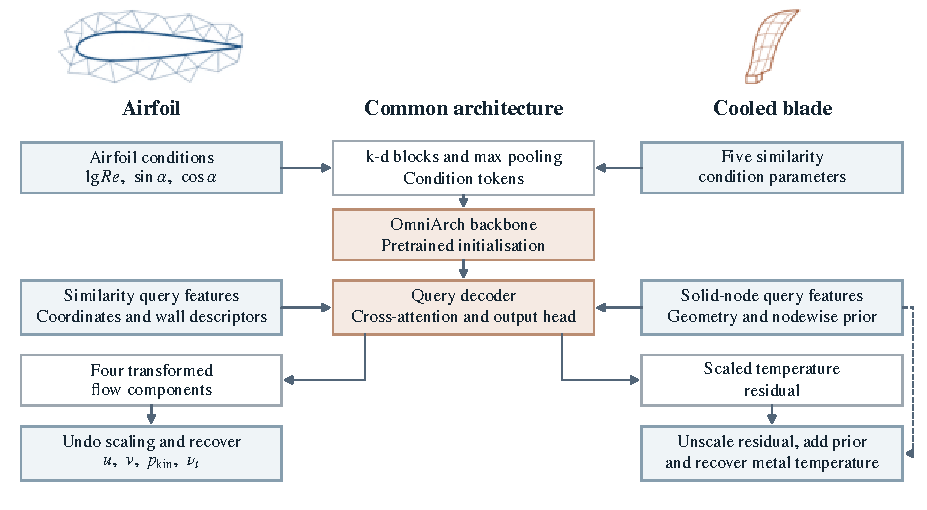
\includegraphics[width=.95\linewidth]{figs/fig2.pdf}
  \caption{翼型与叶片任务的相似变换、共用网格编码及物理场重构。虚线表示在叶片重构时复用逐节点先验。两个任务采用相同架构，分别训练。}
  \label{fig:two-task-workflow}
\end{figure}

为了把数量不一的非结构网格节点组织为固定长度的空间序列，使用 k-d 树递归分块。每次选择节点数最多的块，沿坐标跨度最大的方向按中位数划分。翼型网格划分为 $2048$ 个块，叶片固体网格划分为 $4096$ 个块。翼型编码使用块内全部节点。叶片在预处理时从每块随机选取 $32$ 个节点用于块编码，同一网格上的各工况共用这组采样节点。

翼型空间块的节点特征包括二维坐标、对数壁距、壁面法向的两个分量和壁面标记，非壁面节点的法向分量取零。叶片节点特征包括三维坐标、距旋转轴的径向距离、到最近流体节点和气侧表面节点的两项对数距离。叶片的查询向量在这六个几何分量后加入标准化的温度先验。

先对块内节点逐点应用多层感知机，再按特征分量取最大值，得到与块内节点顺序无关的聚合特征\citep{Qi2017PointNet}。聚合特征映射为块 token，并叠加块中心的傅里叶位置编码。翼型工况沿用第~\ref{subsec:airfoil-similarity}~节的标准化方式，叶片的五个工况参数分别除以 $S_0$ 中 $600\,\mathrm{K}$ 工况的对应值。每个工况标量映射为一个工况 token，与空间块 token 和一个可训练的汇总 token 拼接，共同进入宽度为 $1024$、包含 $16$ 个注意力头的主干。主干的八个块及末端归一化由 OmniArch-base\citep{Chen2025OmniArch} 的前八个块与末端归一化初始化。主干与新增的网格嵌入、工况嵌入、查询解码器和输出头在各自任务上共同训练。

解码时，将查询节点的特征嵌入为查询向量，再通过一层交叉注意力\citep{Vaswani2017}读取已编码的空间块和工况信息。输出头在每个查询位置返回翼型的四个标准化场分量，或叶片的一个缩放后温度残差。推理对每个目标工况执行一次编码，随后分批查询并复用同一编码序列，直至恢复全部目标节点的物理场。

物理信息神经网络将控制方程的残差纳入损失函数\citep{Raissi2019}。本文通过相似变换和温度先验构造监督训练目标。设一次采样中有 $N_q$ 个查询节点和 $C$ 个输出分量，第 $i$ 个节点的第 $c$ 个分量的训练目标与预测分别为 $y_{ic}$ 和 $\widehat y_{ic}$。给定查询点权重 $w_i$ 和分量权重 $a_c$，采用加权均方误差
\begin{equation}
  \label{eq:weighted-training-loss}
  \mathcal{L}=
  \frac{\displaystyle\sum_{i=1}^{N_q} w_i
    \left[\frac{1}{C}\sum_{c=1}^{C}a_c
      (\widehat y_{ic}-y_{ic})^2\right]}
       {\displaystyle\sum_{i=1}^{N_q}w_i}.
\end{equation}
翼型任务取 $C=4$，相似配置和有量纲配置均在标准化后的四分量输出空间比较误差。每次取一个训练算例的全部壁面节点及至多 $8000$ 个随机非壁面节点。相似配置的壁面节点权重为 $5$、压力分量权重为 $2$，有量纲配置的对应权重均为 $1$，其余权重均取 $1$。有量纲配置的七维查询向量采用两个来流速度分量和对数壁距。因此，第~\ref{sec:airfrans-results}~章比较两套完整训练配置。

叶片任务取 $C=1$，采用式~\eqref{eq:blade-training-residual} 给出的残差除以 $\sigma_\theta$ 作为训练目标。每次从一个训练工况选取 $49152$ 个固体节点，$w_i$ 与 $a_c$ 均取 $1$。两个任务均用 AdamW\citep{Loshchilov2019} 优化，学习率线性预热后按余弦规律衰减。翼型使用随机种子 $0$ 至 $2$ 分别训练和评价。叶片使用随机种子 $0$ 至 $4$ 分别训练，在物理温度空间按节点平均各模型的预测，再计算集成温度场的误差。
% 定稿时在附录汇总学习率、优化步数、设备，以及复现脚本与原训练设置的区别。

\section{AirfRANS 基准上的雷诺数外推}\label{sec:airfrans-results}
\sectionbudget{4}

\subsection{基准划分与比较设置}\label{subsec:airfrans-setup}
\subsectionbudget{0.75}

采用 AirfRANS 的同一雷诺数划分评价相似配置和有量纲配置。两套配置均在 $Re\in[3\times10^6,\,5\times10^6]$ 内的 $504$ 个算例上训练，在区间外的 $496$ 个算例上测试。图~\ref{fig:airfrans-operating-split} 给出低于训练区间的 $254$ 个和高于训练区间的 $242$ 个测试算例。雷诺数根据官方划分清单中的来流速度，以及第~\ref{subsec:airfoil-similarity}~节给出的弦长和运动黏度计算。每个算例均提供翼型几何和来流工况。

\begin{figure}[width=\linewidth,pos=htbp]
  \centering
  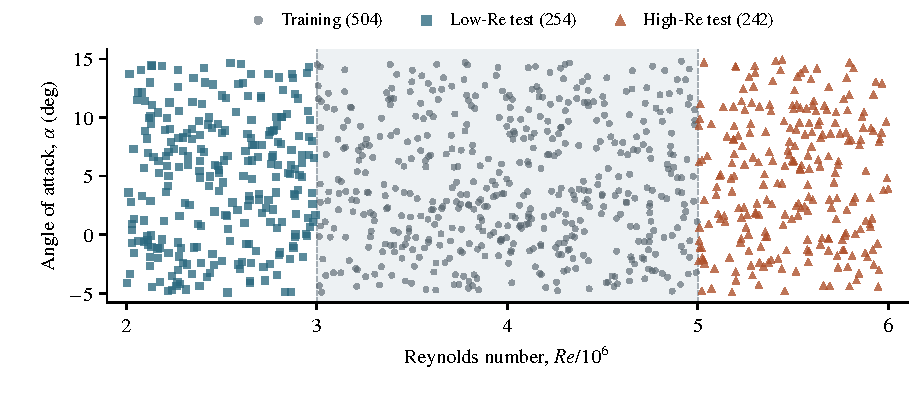
\includegraphics[width=.95\linewidth]{figs/fig3.pdf}
  \caption{AirfRANS 算例在雷诺数与攻角上的分布。每个点对应官方雷诺数划分中的一个算例，阴影带标出训练区间。}
  \label{fig:airfrans-operating-split}
\end{figure}

两套配置采用相同的主干初始化和训练进度。表~\ref{tab:airfrans-configurations} 汇总第~\ref{subsec:mesh-to-field}~节所述表征和损失权重的差异。

\begin{table}[width=.96\linewidth,cols=3,pos=htbp]
  \caption{AirfRANS 对比中的有量纲配置和相似配置。}
  \label{tab:airfrans-configurations}
  \begin{tabular*}{\tblwidth}{@{}LCC@{}}
    \toprule
    设置 & 有量纲配置 & 相似配置 \\
    \midrule
    工况向量 & $(Re/10^6,\,\alpha/10,\,U_\infty/60)$
      & $(\lg Re,\,\sin\alpha,\,\cos\alpha)$ \\
    查询表征
      & \makecell[c]{来流速度分量\\和壁距的对数}
      & \makecell[c]{攻角特征和\\按雷诺数缩放的壁距} \\
    查询维数 & $7$ & $8$ \\
    标准化前的场预测目标 & 有量纲场 & 相似变量场，见式~\eqref{eq:airfoil-forward} \\
    壁面节点权重 & $1$ & $5$ \\
    压力分量权重 & $1$ & $2$ \\
    \bottomrule
  \end{tabular*}
  \par\smallskip
  \begin{minipage}{\tblwidth}
    \footnotesize
    有量纲工况向量中的攻角数值以度为单位，来流速度以 \(\mathrm{m/s}\) 为单位。
  \end{minipage}
\end{table}

两套配置的预测均恢复为有量纲的物理场，再按同一套 AirfRANS 气动力后处理流程\citep{Bonnet2022AirfRANS}计算升力系数。对随机种子 $0$、$1$ 和 $2$，分别在完整测试集上计算升力系数的相对 $L_2$ 误差，并汇报三个误差的均值和标准差。Spearman 秩相关系数 $\rho_L$ 用于比较预测与参考升力系数在各测试算例间的排序。

\subsection{升力预测精度}\label{subsec:airfrans-errors}
\subsectionbudget{2.00}

记 $\Gamma_w$ 为翼型表面，$\mathbf{n}$ 为从翼面指向流体的单位法向量，$\mathbf{s}_w$ 为按这一法向约定计算的黏性牵引除以密度。升力方向为 $\mathbf{e}_L=(-\sin\alpha,\cos\alpha)$。对单位展向长度，升力系数为
\begin{equation}
  \label{eq:airfrans-lift}
  C_L=\frac{2}{U_\infty^2 L}
      \int_{\Gamma_w}
      \left(-p_{\mathrm{kin}}\mathbf{n}+\mathbf{s}_w\right)
      \cdot\mathbf{e}_L\,\mathrm{d}\ell .
\end{equation}
离散积分时，先将压力、法向量和黏性牵引的节点值平均到表面线段，再按线段长度加权求和。算例的弦长为 $L=1\,\mathrm{m}$。评价时沿用基准的处理方式，将预测的壁面速度和湍流运动黏度置零。黏性牵引由壁面速度梯度与分子运动黏度计算。参考场和预测场均使用相同的气动力计算流程。

对固定的翼型几何和工况，令 $\delta$ 表示预测值减去参考值。对式~\eqref{eq:airfrans-lift} 的预测积分与参考积分作差，得到单个算例的升力系数误差。为衡量整套测试集的误差，将各算例的预测与参考升力系数分别汇成向量 $\widehat{\mathbf{C}}_L$ 和 $\mathbf{C}_L$，则有
\begin{equation}
  \label{eq:airfrans-lift-error}
  \begin{aligned}[b]
    &\delta C_L=\frac{2}{U_\infty^2 L}
      \int_{\Gamma_w}
        \left(-\delta p_{\mathrm{kin}}\mathbf{n}+\delta\mathbf{s}_w\right)
        \cdot\mathbf{e}_L\,\mathrm{d}\ell, \\
    &\varepsilon_{C_L}
      =\frac{\left\|\widehat{\mathbf{C}}_L-\mathbf{C}_L\right\|_2}
             {\left\|\mathbf{C}_L\right\|_2}.
  \end{aligned}
\end{equation}
相对误差的分子对各算例的升力系数绝对误差平方求和后开方，分母使用同一测试集中所有参考升力系数的向量范数。

在相同的测试集上，相似配置使升力系数相对 $L_2$ 误差的均值从 $0.0514$ 降至 $0.0182$，降幅约为 $65\%$（表~\ref{tab:airfrans-lift}）。相似配置的 Spearman 秩相关系数为 $0.9996$，表明在这 $496$ 个算例中，预测与参考升力系数的排序高度一致。相对误差衡量系数大小的吻合程度，秩相关衡量算例之间的排序一致性。

\begin{table}[width=.9\linewidth,cols=4,pos=htbp]
  \caption{AirfRANS 的 496 个雷诺数外推算例上的升力预测精度。}
  \label{tab:airfrans-lift}
  \begin{tabular*}{\tblwidth}{@{}LCCC@{}}
    \toprule
    配置 & 种子数 & $C_L$ 相对 $L_2$ 误差 & Spearman $\rho_L$ \\
    \midrule
    有量纲配置 & $3$ & $0.0514\pm0.0038$ & \textemdash \\
    相似配置 & $3$ & $0.0182\pm0.0026$ & $0.9996$ \\
    \bottomrule
  \end{tabular*}
  \par\smallskip
  \begin{minipage}{\tblwidth}
    \footnotesize
    每套配置均在 $504$ 个算例上训练。相对 $L_2$ 误差见式~\eqref{eq:airfrans-lift-error}，
    按随机种子 $0$、$1$ 和 $2$ 汇报均值 $\pm$ 标准差。$\rho_L$ 取自实验汇总，
    横线表示该配置暂无对应的秩相关数值。
  \end{minipage}
\end{table}

图~\ref{fig:airfrans-lift-parity} 预留用于逐算例展示表~\ref{tab:airfrans-lift} 的汇总误差。两套配置的子图使用共同的坐标范围，并区分两个外推区间。

\begin{figure}[width=\linewidth,pos=htbp]
  \centering
  \figureguide{逐算例升力对比（待绘图）}
    {两套配置在种子 0、1、2 下的逐算例 \texttt{metrics.json}，其中含配对的参考与预测 $C_L$。按算例编号关联雷诺数划分。}
    {每套配置绘制一个子图，横轴为参考 $C_L$，纵轴为预测 $C_L$。采用相同坐标范围和等比例坐标轴，画出等值线，用不同标记区分低、高 $Re$ 算例。}
    {每个子图、每个种子应包含 496 对数据（低 $Re$ 为 254 对，高 $Re$ 为 242 对）。按式~\eqref{eq:airfrans-lift-error} 重算每个种子的误差，核对表~\ref{tab:airfrans-lift} 舍入后的均值与标准差。}
  \fbox{\parbox[c][42mm][c]{.88\linewidth}{\centering\strut}}
  \caption{拟比较两个外推区间内的预测与参考升力系数。}
  \label{fig:airfrans-lift-parity}
\end{figure}

式~\eqref{eq:airfrans-lift-error} 中的压力贡献同时取决于局部压力误差和表面法向。翼面不同位置的压力偏差在积分时可能相互加强或抵消。因此，升力误差较小时，局部压力场仍可能有偏差。图~\ref{fig:airfrans-pressure-fields} 预留用于并列比较压力场与表面压力系数曲线。训练区间两侧各选一个算例，选取规则为该侧雷诺数最接近中位数的算例。

\begin{figure}[width=\linewidth,pos=htbp]
  \centering
  \figureguide{压力场与表面曲线（待绘图）}
    {AirfRANS 参考网格与节点压力、对应的模型预测压力，以及各选定算例的表面坐标、来流速度和升力误差。}
    {每个 $Re$ 区间一行。选取最接近区间中位数的算例，若并列则按算例编号确定。参考与预测 $p_{\mathrm{kin}}$ 共用色标，有符号误差使用以零为中心的色标，并绘制上下表面 $C_p$ 随 $x/L$ 的曲线。}
    {每行注明算例编号、$Re$、攻角、配置、种子及升力误差。逐节点确认误差等于预测减参考，并按 $C_p=2p_{\mathrm{kin}}/U_\infty^2$ 核对两条曲线。}
  \fbox{\parbox[c][62mm][c]{.88\linewidth}{\centering\strut}}
  \caption{拟比较代表性低雷诺数和高雷诺数算例的压力场与表面压力。}
  \label{fig:airfrans-pressure-fields}
\end{figure}

\subsection{外推性能分析与推理耗时}\label{subsec:airfrans-comparison}
\subsectionbudget{1.25}

表~\ref{tab:airfrans-lift} 的误差降幅对应两套完整配置。相似配置的查询向量为八维，有量纲配置为七维。两套配置的壁面节点权重和压力分量权重分别为 $(5,2)$ 和 $(1,1)$。因此，比较结果反映了场变量表示、查询特征和损失权重共同变化后的效果。使用当前实现重新评价原始检查点，复现了两套配置的误差均值和标准差。

将空间块 token 替换为另一翼型的对应 token，用以检查编码后的几何信息对预测的影响。实验记录的输出变化约为 $0.24$，对应标准化输出的量级约为 $0.72$。这一响应表明，翼型预测对通过空间块 token 输入的几何信息敏感。第~\ref{subsec:blade-discussion}~节进一步讨论同一网格上的叶片任务对编码信息的依赖。

实验汇总记录的单算例流场预测耗时约为 $0.22\,\mathrm{s}$，RANS 计算耗时约为 $25\,\mathrm{min}$。在当前实现中，计时对应一个模型检查点的一次预测调用，调用前后均执行 GPU 同步。计时范围包含加载已预处理的算例、流场编码与解码，以及将有量纲的预测结果传回主机。输出文件写入和气动力后处理在计时结束后执行。
% 根据原始计时记录核对两项耗时对应的硬件、网格规模和计时边界，再计算加速比。

\section{冷却涡轮叶片的温度外推}\label{sec:blade-results}
\sectionbudget{4}

\subsection{工程算例与对照方法}\label{subsec:blade-setup}
\subsectionbudget{1.00}
% 待根据原 CFX 工程核对并补充材料物性及完整边界条件。

叶片研究采用同一冷却涡轮转子叶片的七个已收敛 CFX 共轭传热算例。各工况的温度场均在同一套包含 $3{,}304{,}055$ 个固体节点的网格上评价。气侧表面从 CFX 的 \emph{surface Shadow} 区域提取，包含 $95{,}837$ 个固体节点。在全部七个工况中，重建表面的面积加权平均温度与 CFX 记录值的差异均在 $3\times10^{-5}\,\mathrm{K}$ 以内。提取的节点坐标在各工况间一致，为逐节点构造先验提供了对应关系。

表~\ref{tab:blade-cases} 列出了五个训练算例、其中用于拟合先验的三个算例，以及两个高温测试算例。两个测试工况均使用同样的三个低温参考场构造先验。两个训练算例的 $T_g$ 同为 $600\,\mathrm{K}$，但冷气进口总温不同，先验拟合使用表中指定的那个算例。

\begin{table}[width=.92\linewidth,cols=6,pos=htbp]
  \caption{七个冷却叶片算例的进口总温及其用途。}
  \label{tab:blade-cases}
  \begin{tabular*}{\tblwidth}{@{}LCCCCC@{}}
    \toprule
    算例 ID & $T_g$（K） & $T_c$（K） & 训练 & 拟合先验 & 测试 \\
    \midrule
    e3-model-600K\_001  &  600.0 & 334.5 & 是 & 是 & \textemdash \\
    e3-model-800K\_001  &  800.0 & 445.0 & 是 & 是 & \textemdash \\
    e3-model-1000K\_001 & 1000.0 & 557.5 & 是 & 是 & \textemdash \\
    e3-unmodel-600K\_001 & 600.0 & 401.4 & 是 & \textemdash & \textemdash \\
    e3\_redown40\_001   &  683.8 & 344.0 & 是 & \textemdash & \textemdash \\
    e3-model-1200K\_001 & 1200.0 & 669.0 & \textemdash & \textemdash & 是 \\
    e3-1616K\_001       & 1616.0 & 901.0 & \textemdash & \textemdash & 是 \\
    \bottomrule
  \end{tabular*}
\end{table}

在同一网格上比较三种温度重构方法。直接相似换算沿用 $T_g$ 最接近目标工况的先验算例的无量纲温度场，两个测试工况均选用 $1000\,\mathrm{K}$ 算例。逐节点线性先验将目标 $T_g$ 代入式~\eqref{eq:blade-linear-prior} 求值。完整模型在该先验上叠加网络学习的残差。三种方法均利用目标工况的 $T_g$ 和 $T_c$，通过式~\eqref{eq:blade-temperature-similarity} 恢复金属温度。

\subsection{固体域温度预测误差}\label{subsec:blade-errors}
\subsectionbudget{1.75}

评价完整模型时，先将随机种子 $0$ 至 $4$ 训练得到的五个模型的预测温度逐节点平均，再与 CFX 参考场计算误差。记 $\widehat T_i^{(m)}$ 为模型 $m$ 在固体节点 $i$ 上的预测温度，$T_i$ 为 CFX 参考温度，$N_s$ 为固体节点数。取 $M=5$，集成预测及其平均绝对误差为
\begin{equation}
  \label{eq:blade-ensemble-mae}
  \begin{aligned}[b]
    &\widehat T_i^{\,\mathrm{ens}}
      =\frac{1}{M}\sum_{m=1}^{M}\widehat T_i^{(m)}, \\
    &\mathrm{MAE}_T^{\,\mathrm{ens}}
      =\frac{1}{N_s}\sum_{i=1}^{N_s}
       \left|\widehat T_i^{\,\mathrm{ens}}-T_i\right|.
  \end{aligned}
\end{equation}

MAE 对所有固体节点等权，并按测试工况分别计算。

两个测试工况下，完整模型的全固体节点 MAE 均最低，见表~\ref{tab:blade-temperature-mae}。在 $T_g=1200\,\mathrm{K}$ 时，直接相似换算、逐节点线性先验和残差修正后的 MAE 分别为 $5.32$、$1.84$ 和 $1.56\,\mathrm{K}$。在 $T_g=1616\,\mathrm{K}$ 时，对应数值为 $20.96$、$5.34$ 和 $4.90\,\mathrm{K}$。后一工况的 $T_c=901\,\mathrm{K}$，由式~\eqref{eq:blade-temperature-error} 可知，集成预测的无量纲温度 MAE 约为 $4.90/715\approx0.00685$。

\begin{table}[width=.9\linewidth,cols=3,pos=htbp]
  \caption{两个高温外推工况下的叶片金属温度预测误差。}
  \label{tab:blade-temperature-mae}
  \begin{tabular*}{\tblwidth}{@{}LCC@{}}
    \toprule
    \multirow[c]{2}{*}[-\dimexpr(\aboverulesep+\belowrulesep+\cmidrulewidth)/2\relax]{方法}
    & \multicolumn{2}{c}{全固体节点 MAE（K）} \\
    \cmidrule(l){2-3}
    & $T_g=1200\,\mathrm{K}$ & $T_g=1616\,\mathrm{K}$ \\
    \midrule
    直接相似换算 & $5.32$ & $20.96$ \\
    逐节点线性温度先验 & $1.84$ & $5.34$ \\
    先验与网络残差 & $1.56$ & $4.90$ \\
    \bottomrule
  \end{tabular*}
  \par\smallskip
  \begin{minipage}{\tblwidth}
    \footnotesize
    MAE 对全体固体节点等权。两种基线直接在各自的重构场上计算误差，
    最后一行采用式~\eqref{eq:blade-ensemble-mae} 的逐节点集成预测。
  \end{minipage}
\end{table}

全固体域 MAE 衡量整片叶片的平均误差。局部热评估还要考察高温区域的温度和位置。最高温度偏差 $\max_i\widehat T_i-\max_i T_i$ 是预测场与参考场各自峰值的差。在参考热点处的温度偏差则比较同一节点上的两种温度。热点位移定义为预测场与参考场中最高温度节点之间的欧氏距离。气侧表面 MAE 衡量该界面上节点的温度误差。表~\ref{tab:blade-local-errors} 预留用于比较局部误差，图~\ref{fig:blade-temperature-fields} 预留用于展示对应的温度场。

\begin{table}[width=.96\linewidth,cols=5,pos=htbp]
  \displayguide{\tblwidth}{局部温度与热点误差（待填表）}
    {两个叶片测试工况下三种方法的逐算例 \texttt{metrics.json}。短横线表示等待评估的数值。}
    {使用直接换算、线性先验与五种子平均场的结果，三列依次填入 \texttt{outer\_mae\_K}、\texttt{Tmax\_err\_K} 和 \texttt{hotspot\_dist\_mm}。}
    {逐工况、逐方法核对全部 18 个值。气侧表面 MAE 是表面节点绝对误差的平均值（K）。峰值偏差为 $\max\widehat T-\max T$（K）。热点位移为两个峰值节点之间的距离（mm）。}
  \caption{两个叶片测试工况的局部金属温度与热点误差。}
  \label{tab:blade-local-errors}
  \begin{tabular*}{\tblwidth}{@{}LLCCC@{}}
    \toprule
    $T_g$（K） & 方法 & 气侧 MAE（K） & 峰值偏差（K） & 热点位移（mm） \\
    \midrule
    \multirow[c]{3}{*}{1200}
      & 直接相似换算 & \textemdash & \textemdash & \textemdash \\
      & 逐节点线性先验 & \textemdash & \textemdash & \textemdash \\
      & 先验加学习残差 & \textemdash & \textemdash & \textemdash \\
    \midrule
    \multirow[c]{3}{*}{1616}
      & 直接相似换算 & \textemdash & \textemdash & \textemdash \\
      & 逐节点线性先验 & \textemdash & \textemdash & \textemdash \\
      & 先验加学习残差 & \textemdash & \textemdash & \textemdash \\
    \bottomrule
  \end{tabular*}
\end{table}

\begin{figure}[width=\linewidth,pos=htbp]
  \centering
  \figureguide{叶片温度场与热点（待绘图）}
    {固体节点坐标与气侧表面网格、CFX 节点温度，以及 1200 和 1616\,K 工况对应的五种子平均温度场。}
    {每个工况一行。从同一视角展示 CFX 温度、集成温度和绝对误差（K）。同一行内的两幅温度场共用色标。标明气侧表面和截面，在叶片上标出两个峰值节点。}
    {先逐节点平均五个预测，再计算 $|\widehat T^{\rm ens}-T|$。全固体节点的均值在 1200\,K 和 1616\,K 工况下应分别舍入为 1.56\,K 和 4.90\,K。用表~\ref{tab:blade-local-errors} 核对峰值节点间距。}
  \fbox{\parbox[c][62mm][c]{.88\linewidth}{\centering\strut}}
  \caption{拟对比参考温度场与集成温度场，并展示绝对误差和热点位置。}
  \label{fig:blade-temperature-fields}
\end{figure}

\subsection{温度先验的贡献与适用范围}\label{subsec:blade-discussion}
\subsectionbudget{1.25}

相对于直接相似换算，大部分 MAE 的改善来自逐节点先验。在 $1616\,\mathrm{K}$ 工况下，线性先验使 MAE 降低 $15.62\,\mathrm{K}$，网络残差修正进一步降低 $0.44\,\mathrm{K}$。在 $1200\,\mathrm{K}$ 工况下，两步改善分别为 $3.48\,\mathrm{K}$ 和 $0.28\,\mathrm{K}$。

在原始叶片模型上扰动编码输入，以检查残差预测对这些输入的敏感性。将空间块 token 替换为噪声、置零，或将五个全局工况参数减半，输出变化均小于 $10^{-8}$，而该模型的输出量级约为 $10^{-3}$。这些扰动保留了查询向量中的逐节点温度先验。全部叶片工况共用同一网格，先验已在各节点提供随工况变化的信息。扰动后的微小响应表明训练后的叶片网络对该几何上的先验进行逐节点修正。

在翼型任务中（第~\ref{subsec:airfrans-comparison}~节），换用另一几何的空间块 token 后，在翼型输出尺度下可测得相应的变化（图~\ref{fig:encoder-diagnostics}）。

\begin{figure}[width=\linewidth,pos=htbp]
  \centering
  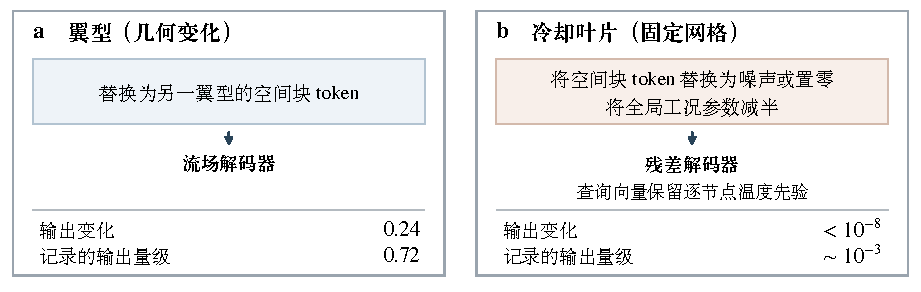
\includegraphics[width=.95\linewidth]{figs/fig7_zh.pdf}
  \caption{翼型与冷却叶片模型对输入扰动的响应。各面板给出输出变化和对应模型自身的输出尺度。叶片在扰动试验中保留查询节点的逐节点温度先验。}
  \label{fig:encoder-diagnostics}
\end{figure}

式~\eqref{eq:blade-temperature-similarity} 中的进口温差给出了从无量纲温度换算至开尔文的尺度。物性与界面换热随工况改变时，无量纲温度分布仍可能发生变化\citep{Cartlidge2024}。两个测试工况表明，在给定的转子叶片上拟合这种变化能够改善温度预测。若应用于其他叶型或网格，需要重新建立固体节点的对应关系，或在新网格上拟合先验。

\section{结论}\label{sec:conclusion}
\sectionbudget{1}

OmniArch-Aero 将面向任务的相似表示引入非结构网格上的工况外推。翼型模型在相似变量空间预测流场，用于雷诺数外推。叶片模型结合逐节点温度先验与网络学习的残差，重构更高进口温度工况下的金属温度场。两个任务采用相同的网格到场映射架构，并分别训练。

在同一批 $496$ 个 AirfRANS 外推算例上，升力系数相对 $L_2$ 误差由有量纲配置的 \mbox{$0.0514\pm0.0038$} 降至相似配置的 \mbox{$0.0182\pm0.0026$}，数值为三次训练结果的均值 $\pm$ 标准差（表~\ref{tab:airfrans-lift}）。在冷却叶片的 $T_g=1616\,\mathrm{K}$ 工况下，直接相似换算、逐节点线性先验和加入网络残差后的五模型集成预测，在全体固体节点上的平均绝对误差分别为 $20.96$、$5.34$ 和 $4.90\,\mathrm{K}$（表~\ref{tab:blade-temperature-mae}）。

翼型的空间块 token 替换试验表明，预测对编码后的几何信息敏感。在固定网格的叶片算例中，先验贡献了大部分误差降幅，输入扰动的结果支持将网络作用解释为对先验的逐节点修正。将该方法用于其他叶型或网格时，需要建立节点对应关系，或在新网格上拟合先验。跨叶型试验可以进一步检验几何编码在何种条件下有助于提高温度预测精度。

\bibliographystyle{../cmame-num}
\bibliography{../cas-refs}

\end{document}
